\documentclass{kthreport}

\usepackage{hhline}
\usepackage[parfill]{parskip}
\usepackage{subcaption}
\usepackage{placeins}


\title{Classification of ImageNet with Convolutional Neural Networks}
\subtitle{A study in techniques to improve CNN's}
\author{W. Skagerström, T. Price, N. Lindqvist}
\diarienr{Deepl-18 Project}



\begin{document}
\maketitle
\newpage
\begin{abstract}

\noindent
This report is our final piece of work in the course DD2424, Deep Learning in Data Science. The overarching purpose is investigating convolutional neural networks (CNN's) while applying knowledge and techniques which we've acquired in during the course.
\noindent
To thoroughly investigate the topic a CNN will be constructed in the most vanilla way possible. Different architectures is compared to another before moving on with one which performs better in terms of accuracy. In turns the network will be optimized by more sophisticated initialization, changing activation functions and additional additional optimization and regularization such as dropout and batch normalization. The effect of each modification will be documented and analyzed. Lastly, the results is discussed on their own and in context of other imageNet classifiers.
\end{abstract}
\newpage

\section{Introduction}
Image classification is one of the main branches within Computer Vision. The task can be summarized as extracting features from a pixel matrix containing either 1 or 3 channels(for gray-scale or red,green, and blue, respectively). Back in 2012, Convolutional Neural Networks(CNN's) began replacing the previously manually written algorithms for feature detection. (About imageNet being a modern standard:\cite{russakovsky2015imagenet})



\section{Previous work}
Text about previous work, references etc.

\section{Method}
\subsection{Dataset}
The data used was the ImageNet Tiny dataset, which is a reduced variant of the ImageNet set. The Tiny variation consists of 200 different classes. The resolution of the images has been reduced to $64\times64\times3$ (from  $224\times224\times3$). The dataset consists of 100 000 training samples, 10000 validation samples, and 10000 test samples.
\\\\
Below is a small sample of pictures included in the dataset:
\begin{figure}[htbp]
  \centering
  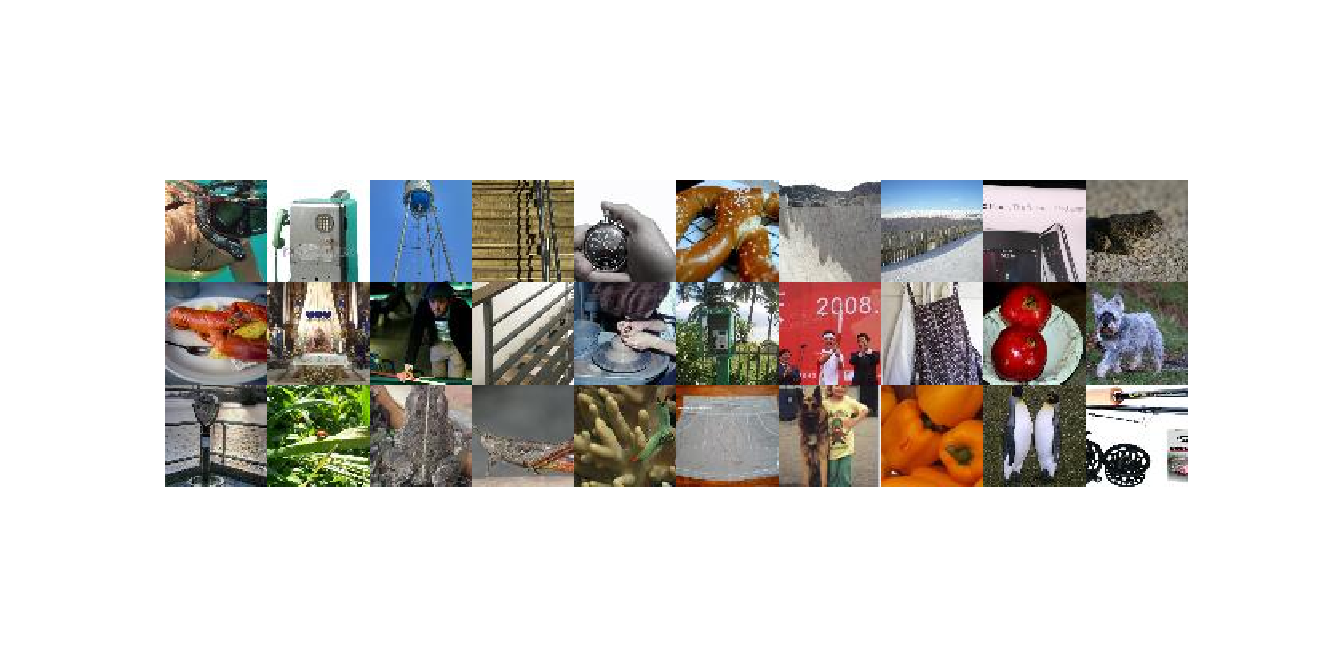
\includegraphics[width=\linewidth]{../images/samples.png}
  \caption[]
  {\small
    30 Samples from the Tiny ImageNet dataset.
  }
  \label{fig:30_samples}
\end{figure}

\FloatBarrier

\subsection{Implementing a CNN}

\subsubsection{Implementation specifics}

The network was written and implemented in Python 3.5.2, using the Keras Framework which runs on top of Tensorflow. Numpy was used for data management and Matplotlib to create the graphs. To assist in training and evaluating the networks, we used Google Cloud services for computation power. The specifications of the hardware used was:
\begin{itemize}
\item 1 x NVIDIA Tesla K80
\item An unspecified dual core CPU (Unknown CPU Platform on the Google Cloud Platform). 
\item 16 GB RAM memory
\item 40 GB Disk space.
\end{itemize}

\subsubsection{Evaluation architectures}

The basis of the CNN architecture is inspired by \cite{NIPS2012_4824}, it is summarized in figure \ref{fig:architecture}. However, it was implemented on the full ImageNet dataset. Inspired by \textbf{insert 3 reports here} we decided to test three configurations, summarized in \ref{table:3_configurations}.

\begin{figure}[htbp]
  \centering
  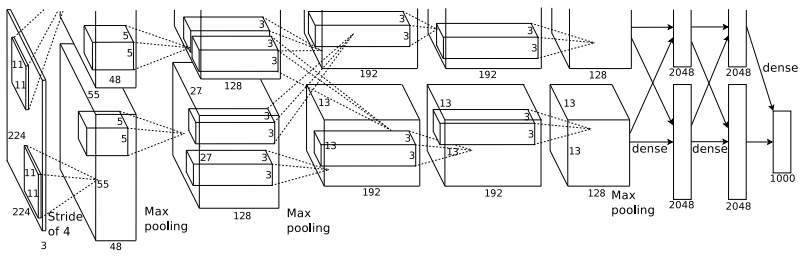
\includegraphics[width=\linewidth]{../images/architecture.jpg}
  \caption[]
  {\small
    Overview of network architecture presented by \cite{NIPS2012_4824}.
  }
  \label{fig:architecture}
\end{figure}

\FloatBarrier

\medskip
\begin{table}[htbp]
\begin{center}
\begin{tabular}{|c|c|c|}

  \hline
  \multicolumn{3}{|c|}{ConvNet Configuration} \\
  \hline

  A & B & C
  \\\hline

  X weight layers & Y weight layers & Z weight layers
  \\\hhline{|=|=|=|}

  \multicolumn{3}{|c|}{input ($64\times64\;RGB\;image$)}
  \\\hline

  conv3-64 & conv3-64 & conv3-64
  \\\hline

  \end{tabular}
\caption[]
{\small
  Configuration of the three different CNNs tested initially. They are inspired from (A) reference, (B) reference and (C) reference.
}
\label{table:3_configurations}
\end{center}
\end{table}

\FloatBarrier


Tests was run with \textbf{insert how tests were run} iterations. Training was done on the entire Tiny Imagenet dataset, containing 100 000 images and their respective labels. The composition of the dataset is 200 classes with 500 images each. The training data is shuffled before the training process begins. For evaluation, the entire validation dataset was used, containing 10000 images. The results of each architecture is presented in section...

\subsubsection{Initialization matters}

Moving on with current architecture of the network we




\subsubsection{First important subtopic}

Lorem Ipsum is simply dummy text of the printing and typesetting industry. Lorem Ipsum has been the industry's standard dummy text ever since the 1500s, when an unknown printer took a galley of type and scrambled it to make a type specimen book. It has survived not only five centuries, but also the leap into electronic typesetting, remaining essentially unchanged. It was popularised in the 1960s with the release of Letraset sheets containing Lorem Ipsum passages, and more recently with desktop publishing software like Aldus PageMaker including versions of Lorem Ipsum.

\section{Results}
Graphs/Tables of trainloss, valloss, accuracies etc. 

\section{Discussion}

\subsection{Evaluation of method}
Thoughts about the method. 

\subsection{Evaluation of results}

Thoughts about the result. 

\subsection{ImageNet state of the art}

Comparing ours to other state of the art networks. 

\section{Conclusion} 
Final thoughts, future research, improvements etc. 

\bibliography{references}{}
\bibliographystyle{plain}

\end{document}
